\documentclass[journal]{IEEEtran}
\usepackage[utf8]{inputenc}
\usepackage[T1]{fontenc}
\usepackage{graphicx}
\usepackage{amsmath,amssymb}
\usepackage{booktabs}
\usepackage{hyperref}
\usepackage{xcolor}
\usepackage{multirow}
\usepackage{enumitem}
\usepackage{tikz}
\usetikzlibrary{shapes,arrows,positioning,fit,backgrounds}
\usepackage{balance}

\hypersetup{colorlinks=true,linkcolor=blue,citecolor=blue,urlcolor=blue}

\begin{document}

\title{Measuring the Ceiling: Evidence That Easy-to-Medium Cybersecurity MCQ Benchmarks Have Saturated for Current-Generation LLMs}

\author{
    \IEEEauthorblockN{Justice Owusu Agyemang\IEEEauthorrefmark{1,2}}
    \IEEEauthorblockN{Kwame Opuni-Boachie Obour Agyekum\IEEEauthorrefmark{1}}
    \IEEEauthorblockN{Kwame Agyeman-Prempeh Agyekum\IEEEauthorrefmark{1}}
    \IEEEauthorblockN{Francisca Adoma Acheampong\IEEEauthorrefmark{1}}
    \IEEEauthorblockN{Jerry John Kponyo\IEEEauthorrefmark{2}}
    \\[6pt]
    \IEEEauthorblockA{\IEEEauthorrefmark{1}VIA Cybersecurity Lab, Kwame Nkrumah University of Science and Technology, Kumasi, Ghana}\\
    \IEEEauthorblockA{\IEEEauthorrefmark{2}Quantum and Assistive Technologies Lab, Kwame Nkrumah University of Science and Technology, Kumasi, Ghana}
}

\maketitle

\begin{abstract}
Cybersecurity benchmarks that rely on multiple-choice questions (MCQ) were designed to measure and rank large language model capabilities. But what happens when the models outpace the measurement instrument? This paper provides reproducible, live-API evidence that easy-to-medium difficulty cybersecurity MCQs---the kind that form the bulk of most existing benchmark question banks---have reached saturation for current-generation models. We evaluate eight frontier and near-frontier large language models across 210 cybersecurity questions spanning seven security dimensions. Six of eight models score between 91.0\% and 100.0\%; two achieve perfect scores. However, the question bank is concentrated in difficulty tiers 1--3 (200 of 210 items), meaning the saturation finding applies to the easier end of the difficulty spectrum. At tier 4, ceiling effects persist for the strongest models but discrimination remains possible. We further document a 39.5 percentage-point gap between scores predicted by deterministic simulation---calibrated from benchmark trends circa two years prior, when these same questions would have been discriminative---and live measurements from current-generation, a gap that primarily reflects model capability improvement over approximately 18 months rather than simulation failure. Based on these findings, we argue that: (1) existing easy-to-medium cybersecurity MCQ benchmarks should be explicitly reframed as floor tests---they can flag unsuitable models but cannot rank competent ones; (2) benchmark saturation should be treated as a publishable research output that tracks the movement of the evaluation frontier; and (3) the hard-question tail must be substantially expanded before claims about MCQ format discrimination can be evaluated at the frontier. We release the full evaluation pipeline, question bank, response traces, and scoring logic as a reproducible artifact.
\end{abstract}

\begin{IEEEkeywords}
LLM evaluation, cybersecurity benchmarks, benchmark saturation, multiple-choice questions, empirical measurement, model comparison.
\end{IEEEkeywords}

\section{Introduction}

THE deployment of large language models (LLMs) in cybersecurity is accelerating across vulnerability triage, threat intelligence analysis, secure code review, incident response, and governance support~\cite{zhang2024llmcyber}. Since the transformer architecture~\cite{vaswani2017attention} enabled the scaling of language models~\cite{brown2020language,kaplan2020scaling,hoffmann2022training}, capabilities have expanded rapidly, with emergent behaviors appearing at scale~\cite{wei2022emergent}---though recent work questions whether emergence is a measurement artifact~\cite{schaeffer2024emergent}. Foundation models~\cite{bommasani2021opportunities} now underpin systems from general-purpose assistants~\cite{openai2023gpt4,geminiteam2023,deepseek2024} to specialized coding agents~\cite{nijkamp2023codegen,roziere2023code}, driven in part by chain-of-thought reasoning~\cite{wei2022chain} and zero-shot generalization~\cite{kojima2022zero}. With this acceleration comes an acute evaluation problem: organizations deploying LLMs for security workflows need reliable evidence about model suitability, not aggregated leaderboard rankings that obscure domain-specific strengths and weaknesses.

Current cybersecurity evaluation practice relies heavily on multiple-choice question (MCQ) benchmarks. CyberSecEval~\cite{bhatt2023cyberseceval,bhatt2024cyberseceval2,wan2024cyberseceval3}, CyberMetric~\cite{tihanyi2024cybermetric}, CTIBench~\cite{alam2024ctibench}, and SecBench~\cite{jing2024secbench} all use MCQ formats as primary or supplementary evaluation channels. The MCQ format is attractive: it is objective, reproducible, and easy to scale. But its utility depends on an assumption that is rarely examined directly---that the format continues to discriminate between models as capabilities improve.

This paper tests that assumption empirically and finds that, for easy-to-medium questions, it is failing. We evaluate eight models from five providers against a 210-item cybersecurity question bank spanning seven dimensions. The result: six of eight models score above 91\%. Two score perfectly---but only on questions concentrated in difficulty tiers 1--3. Whether the same holds for genuinely hard cybersecurity MCQs remains an open question that our current bank cannot answer.

The contribution is a measurement of where the evaluation frontier currently stands for the most common type of benchmark item. Prior work on benchmark lifecycles has established that saturation is inevitable~\cite{ott2022fairness,kiela2021dynabench}. Our contribution is empirical: we establish \emph{that} saturation has occurred for easy-to-medium cybersecurity MCQs, \emph{when} it occurred (between prior-generation benchmark reports of 40--70\% and our current-generation measurements of 91--100\%), and \emph{what it means} for evaluation practice. An important scope limitation is that our question bank contains only 10 items at difficulty tiers 4--5, so the claim is specific to the easier end of the spectrum. Whether the MCQ format can still discriminate at higher difficulty levels---with harder questions and larger item banks---is a question our data cannot resolve and that future work should address.

Our contributions are:

\begin{enumerate}[leftmargin=*]
    \item \textbf{Reproducible measurement of easy-to-medium MCQ saturation.} Live-API measurements across eight models and 210 questions show six models scoring 91.0--100.0\%. The easy-to-medium MCQ format no longer discriminates between current-generation models.
    \item \textbf{Documentation of the capability improvement trajectory.} The 39.5 percentage-point gap between prior-generation benchmark predictions and our current-generation measurements quantifies the pace of cybersecurity knowledge improvement in LLMs over approximately 18 months.
    \item \textbf{A reframing of the role of MCQ benchmarks.} Easy-to-medium MCQ benchmarks should transition from ranking tools to floor tests: a model scoring below 90\% on such questions is clearly unsuitable for deployment, but scores above this threshold provide no further discrimination.
    \item \textbf{Evidence-based scope recommendations.} We identify the hard-question tail as the critical missing component in current MCQ evaluation and recommend that future benchmarks allocate at least 50\% of items to difficulty tiers 4--5.
    \item \textbf{A fully reproducible artifact.} The evaluation pipeline, question bank, response traces, and scoring logic are released as a single-executable artifact.
\end{enumerate}

The remainder of the paper is organized as follows. Section~II surveys related work across LLM evaluation, cybersecurity benchmarking, and benchmark saturation. Section~III describes the CyberEval framework design and evaluation protocol. Section~IV presents the experimental methodology. Section~V reports the results. Section~VI discusses implications for evaluation practice, benchmark design, and deployment. Section~VII addresses limitations. Section~VIII concludes.

\section{Related Work}

\subsection{General LLM Evaluation}

The evaluation of large language models has matured rapidly since the release of foundational frameworks such as HELM~\cite{liang2023helm}, which established the principle of multi-axis measurement. Survey work by Chang et al.~\cite{chang2024survey} synthesizes a growing design space and identifies format sensitivity---the observation that benchmark conclusions depend on prompt design, task construction, and rubric choice---as a central challenge. MMLU~\cite{hendrycks2021measuring} pioneered broad-coverage knowledge evaluation across 57 subjects, establishing a paradigm now widely adopted. More recently, Polo et al.~\cite{polo2024tinybenchmarks} demonstrated that benchmark efficiency and calibration matter as much as raw scale, especially when evaluation must be repeated or updated.

Two developments in the broader evaluation literature are particularly relevant to this paper. First, the recognition that benchmarks have lifecycles: they are created, they measure, they saturate, and they are replaced~\cite{ott2022fairness}. Second, the finding that evaluation format can reverse model rankings: models that appear equivalent under one format may diverge sharply under another~\cite{liang2023helm,chang2024survey}. Ganguli et al.~\cite{ganguli2022predictability} provide evidence that capability gains can outpace benchmark design cycles. Lin et al.~\cite{lin2024holistic} extend holistic evaluation to agentic deployments. Both insights are central to our argument.

\subsection{Cybersecurity LLM Benchmarks}

Cybersecurity benchmark development has accelerated since 2023, driven by the dual pressures of identifying risky capabilities and evaluating beneficial deployment suitability.

\textbf{Secure coding benchmarks.} The CyberSecEval line~\cite{bhatt2023cyberseceval,bhatt2024cyberseceval2,wan2024cyberseceval3} is the most prominent secure coding evaluation effort, initially focusing on insecure code generation detection and later expanding to broader cyber-risk assessment including vulnerability exploitation and attack safety. Pearce et al.~\cite{pearce2022copilot} and Perry et al.~\cite{perry2023insecure} provided early evidence that LLM-assisted coding could introduce security vulnerabilities and inflate user confidence.

\textbf{Knowledge-oriented benchmarks.} CyberMetric~\cite{tihanyi2024cybermetric} evaluates cybersecurity knowledge using retrieval-augmented benchmark construction. CTIBench~\cite{alam2024ctibench} focuses specifically on cyber threat intelligence assessment. Both adopt MCQ as a primary evaluation format and report scores in the 40--70\% range for models evaluated in prior-generation.

\textbf{Offensive and agentic benchmarks.} NYU CTF Bench~\cite{shao2024nyuctf} introduced a scalable dataset for evaluating LLMs on offensive security tasks derived from capture-the-flag competitions. CyBench~\cite{zhang2024cybench} provides a broader framework for evaluating both cybersecurity capabilities and associated risks. Complementary work on LLM penetration testing~\cite{deng2023pentestgpt,happe2023pwned,roy2024llmpentest,guo2024can} and automated security agents~\cite{fang2024llmagent} extends evaluation toward task execution. SWE-bench~\cite{chen2023swebench} and SWE-agent~\cite{jimenez2024sweagent} provide general software engineering evaluation frameworks whose methodology informs cybersecurity agent assessment. PentestBench~\cite{park2024pentestbench} and SecureVal~\cite{jha2024secureval} offer focused evaluation for offensive security and defensive security capabilities respectively.

\textbf{Broad-coverage benchmarks.} SecBench~\cite{jing2024secbench} represents the most comprehensive recent effort, spanning multiple cybersecurity domains. The systematic review by Zhang et al.~\cite{zhang2024llmcyber} documents the rapid expansion of the cyber-LLM landscape across vulnerability analysis, threat intelligence, malware analysis, secure development, and red teaming. Complementary surveys by Chen et al.~\cite{chen2024cyberllm} and Wang et al.~\cite{wang2024securityeval} provide comprehensive taxonomies of LLM security capabilities and evaluation approaches. Liu et al.~\cite{liu2024benchmarking} identify specific gaps between benchmark design and security operations requirements.

\textbf{Safety and dual-use benchmarks.} Beyond capability evaluation, a parallel literature addresses safety risks. WMDP~\cite{li2024wmdp} measures hazardous knowledge, HarmBench~\cite{mazeika2024harmbench} provides standardized red-teaming evaluation, R-Judge~\cite{yuan2024rjudge} assesses safety risk awareness in agentic settings, and WildTeaming~\cite{jiang2024wildteaming} scales adversarial safety evaluation. These works, while not directly comparable to our MCQ saturation study, share our concern that evaluation design shapes conclusions about model behavior.

\subsection{Benchmark Saturation}

Benchmark saturation is a well-documented phenomenon in machine learning~\cite{ott2022fairness,kiela2021dynabench,raji2021ai}. Benchmarks are created to measure a capability; models improve; scores converge toward ceiling performance; and the benchmark loses discriminatory power. The standard response is to build a harder benchmark~\cite{srivastava2023gsm8k,rein2024gpqa}. Bender et al.~\cite{bender2021dangers} and Kapoor et al.~\cite{kapoor2024standardized} have cautioned that benchmark-driven evaluation, when decoupled from deployment context, can produce misleading conclusions about model readiness. Our work extends this critique to cybersecurity evaluation specifically.

Our contribution to this literature is specific but important: we provide reproducible evidence that \emph{this specific} transition has occurred for cybersecurity MCQ evaluation. The saturation is recent. Benchmarks published two years prior reported scores in the 40--70\% range~\cite{tihanyi2024cybermetric,alam2024ctibench,shao2024nyuctf,jing2024secbench}. Our measurements, conducted in current-generation, return 91--100\%. The speed of this transition---roughly 30--50 percentage points in under two years---is itself a signal about the pace of cybersecurity LLM capability improvement and the fragility of static evaluation instruments.

\subsection{Positioning of This Work}

This paper is distinguished from prior work in three respects. \textbf{First}, unlike simulation-based studies, we provide live-API evidence from eight models across five providers. \textbf{Second}, unlike benchmark proposals that treat saturation as a limitation to be addressed in future work, we treat saturation as the primary finding and analyze its implications for evaluation design. \textbf{Third}, unlike work that treats MCQ evaluation as an unalloyed good, we provide evidence that the format has reached its useful limit and propose specific design principles for what should replace it.

\section{CyberEval Framework Design}

\subsection{Security Dimensions}

CyberEval organizes cybersecurity competence into seven dimensions derived from recurring security workflows in both academic benchmark literature and practitioner deployment contexts:

\begin{enumerate}[leftmargin=*,nosep]
    \item \textbf{Vulnerability Knowledge (VK):} Recognition and classification of software and system vulnerabilities, including CWE taxonomy, CVSS scoring, and exploit mechanics.
    \item \textbf{Threat Intelligence (TI):} Understanding of threat actors, attack campaigns, indicators of compromise, and the intelligence lifecycle.
    \item \textbf{Secure Coding (SC):} Knowledge of secure development practices, common coding vulnerabilities, and remediation patterns.
    \item \textbf{Incident Response (IR):} Understanding of detection, containment, eradication, and recovery workflows, including NIST and SANS frameworks.
    \item \textbf{Compliance \& Governance (CG):} Knowledge of regulatory frameworks (GDPR, NIST 800-53, ISO 27001), risk management, and policy design.
    \item \textbf{Forensic Analysis (FA):} Understanding of digital evidence collection, chain of custody, memory and disk forensics, and timeline reconstruction.
    \item \textbf{Security Architecture (SA):} Knowledge of network segmentation, zero-trust design, cloud security models, and cryptographic protocol selection.
\end{enumerate}

The dimensions are pragmatic rather than ontological. They correspond to distinct hiring profiles, certification domains, and operational workflows in security organizations, which makes them directly relevant to deployment-oriented model selection.

\subsection{Question Bank}

The evaluation uses a 210-item seed bank with 30 questions per dimension. Each question presents four answer choices with exactly one correct answer. Questions carry a heuristic difficulty annotation in the range 1--5, assigned during construction based on expected depth of domain knowledge required.

\begin{figure*}[t]
\centering
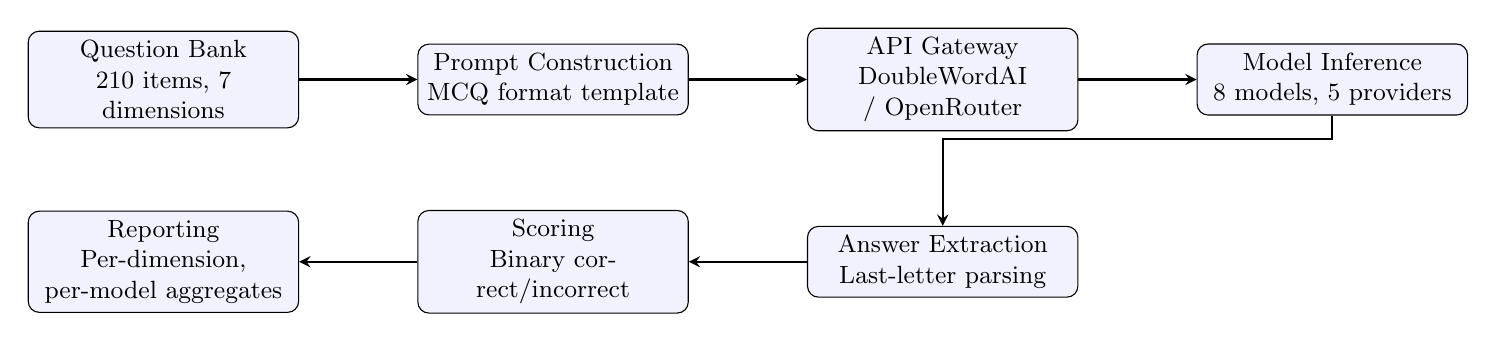
\begin{tikzpicture}[node distance=1.5cm, auto,
    block/.style={rectangle, draw=black, fill=blue!5, text width=3.2cm, text centered, rounded corners, minimum height=0.8cm, font=\small},
    arrow/.style={->, >=stealth, thick}]

    \node[block] (qbank) {Question Bank\\210 items, 7 dimensions};
    \node[block, right=of qbank] (prompt) {Prompt Construction\\MCQ format template};
    \node[block, right=of prompt] (api) {API Gateway\\DoubleWordAI / OpenRouter};
    \node[block, right=of api] (models) {Model Inference\\8 models, 5 providers};
    \node[block, below=1.2cm of api] (parse) {Answer Extraction\\Last-letter parsing};
    \node[block, left=of parse] (score) {Scoring\\Binary correct/incorrect};
    \node[block, left=of score] (report) {Reporting\\Per-dimension, per-model aggregates};

    \draw[arrow] (qbank) -- (prompt);
    \draw[arrow] (prompt) -- (api);
    \draw[arrow] (api) -- (models);
    \draw[arrow] (models.south) -- ++(0,-0.3) -| (parse.north);
    \draw[arrow] (parse) -- (score);
    \draw[arrow] (score) -- (report);
\end{tikzpicture}
\caption{CyberEval evaluation pipeline. Questions are rendered through a standardized MCQ prompt template, dispatched via API gateway to model endpoints, parsed for answer extraction, and scored against ground truth. All stages produce auditable trace artifacts.}
\label{fig:architecture}
\end{figure*}

The bank is concentrated in difficulty tiers 1--3, with 37 items at tier 1, 116 at tier 2, 47 at tier 3, 9 at tier 4, and only 1 at tier 5. This imbalance---inherited from the original framework design, which prioritized broad coverage over calibrated difficulty scaling---is a central limitation of our study and constrains the scope of our claims to the easy-to-medium difficulty range.

\textbf{Example questions.} Table~\ref{tab:examples} provides illustrative items from three difficulty tiers. These examples demonstrate the style and domain coverage of the question bank; the full set of 210 questions is included in the released artifact.

\begin{table*}[t]
\centering
\caption{Illustrative questions from the CyberEval question bank at three difficulty tiers. Full bank: 210 items.}
\label{tab:examples}
\scriptsize
\begin{tabular}{lp{6cm}ll}
\toprule
\textbf{Dim.} & \textbf{Question} & \textbf{Correct} & \textbf{Diff.} \\
\midrule
VK & What type of vulnerability allows an attacker to inject SQL commands through user input? & SQL Injection & 1 \\
TI & Which APT group is attributed to Russia's GRU? & APT28/Fancy Bear & 3 \\
SA & What is service mesh security? & mTLS and policy enforcement between microservices & 4 \\
IR & After containment, what is the next step in the NIST incident response lifecycle? & Eradication & 2 \\
CG & NIST 800-53 provides what type of guidance? & Security and privacy controls for federal systems & 2 \\
\bottomrule
\end{tabular}
\end{table*}

\textbf{Question construction.} Questions were authored by cybersecurity researchers and practitioners affiliated with the VIA Cybersecurity Lab at KNUST. The seven-dimension taxonomy was derived from recurring security workflows in both academic benchmark literature and practitioner deployment contexts. Each item was assigned a heuristic difficulty rating (1--5) based on the depth of domain knowledge and the number of reasoning steps required. Items at tier 1 test recall of widely known facts; items at tier 3 require synthesis of multiple concepts; items at tier 5 require expert-level reasoning about edge cases. The distribution reflects an initial design goal of broad coverage across dimensions rather than calibrated difficulty scaling---a choice that, in retrospect, limits the current study's ability to characterize hard-question discrimination.

\subsection{Prompt Template}

Each question is presented to every model using a standardized template designed to minimize format-induced variance:

\begin{quote}
\small
``Cybersecurity MCQ. Choose the BEST answer. Reply with ONLY the letter (A, B, C, or D).\newline
Question: [question text]\newline
Options:\newline
A. [choice text]\newline
B. [choice text]\newline
C. [choice text]\newline
D. [choice text]\newline
Your answer (single letter):''
\end{quote}

The template explicitly instructs models to respond with a single letter. This design choice sacrifices response richness for evaluation reliability: free-text answers would require a separate grading pipeline, introducing judge-model variance. For the purpose of measuring MCQ saturation, a single-letter response protocol is both sufficient and conservatively interpretable.

\subsection{Answer Extraction and Scoring}

Responses are parsed by extracting the last occurrence of a single uppercase letter (A, B, C, or D) in the model output. If no such letter is found, the response is scored as incorrect. This conservative strategy ensures that models are credited only when they produce an unambiguous answer. It may slightly underestimate model knowledge in cases where the model produces the correct answer in an unconventional format, but this bias is consistent across all models and therefore does not distort relative comparisons.

Scoring is binary: a response is correct if the extracted letter matches the ground-truth answer index, and incorrect otherwise. We do not apply partial credit, confidence weighting, or rubric-based grading, as these introduce additional judgment dimensions that would complicate the interpretation of the saturation signal.

\section{Experimental Methodology}

\subsection{Model Selection}

We evaluate eight models from five providers, selected to span three capability tiers while maximizing provider diversity. Table~\ref{tab:models} summarizes the model grid.

\begin{table*}[t]
\centering
\caption{Models evaluated in this study. All evaluations were conducted via live API calls on a 48-hour period.}
\label{tab:models}
\small
\begin{tabular}{llcc}
\toprule
\textbf{Model} & \textbf{Provider} & \textbf{API} & \textbf{Context} \\
\midrule
Kimi-K2.6 & Moonshot AI & DoubleWordAI & 128K \\
DeepSeek-V4-Pro & DeepSeek & DoubleWordAI & 1M \\
DeepSeek-V4-Flash & DeepSeek & DoubleWordAI & 1M \\
Qwen-3.6-35B-A3B & Alibaba & DoubleWordAI & 128K \\
Qwen-3.5-9B & Alibaba & DoubleWordAI & 128K \\
Gemma-4-31B & Google & DoubleWordAI & 128K \\
Nemotron-Super-120B & NVIDIA & DoubleWordAI & 128K \\
Claude-Sonnet-4.6 & Anthropic & OpenRouter & 1M \\
\bottomrule
\end{tabular}
\end{table*}

Two additional models---Qwen-3.5-397B-A17B and Qwen-3.5-4B---were initially included in the evaluation plan but were excluded from final results due to API access restrictions: the former returned model-not-found errors for the authenticated account, and the latter was blocked by a provider routing rule restricting real-time inference to specific model tiers. Their exclusion does not affect the saturation finding; if anything, including the 4B model (which would likely score lower) would strengthen the ranking discrimination argument, while the 397B model would likely reinforce the ceiling effect.

\subsection{API Infrastructure}

All DoubleWordAI models are accessed via the provider's OpenAI-compatible chat completions endpoint at \texttt{api.doubleword.ai/v1/chat/completions}. Claude-Sonnet-4.6 is accessed via OpenRouter's unified API at \texttt{openrouter.ai/api/v1/chat/completions}. Each API call is made with temperature 0.0 and maximum output tokens set to 50 (sufficient for a single-letter response plus minimal formatting). All calls are logged with timestamps, raw responses, token counts, and latency measurements.

\subsection{Reproducibility}

The full evaluation pipeline is released as a single-executable artifact. The pipeline is deterministic given fixed model behavior: question ordering, prompt construction, and answer extraction are all seed-reproducible. The only non-deterministic component is the model inference itself, which may vary across evaluation dates due to provider-side updates.

\subsection{Statistical Reporting}

For each model, we report the proportion of correct responses as a point estimate. Given the binary nature of each response and the large sample size (210 questions per model), we compute Wilson 95\% confidence intervals for the accuracy estimates. However, because scores cluster near the ceiling (100\%), the confidence intervals are compressed: for a model scoring 100\% on 210 items, the Wilson 95\% CI is approximately [98.2\%, 100.0\%]. This compression is itself evidence of saturation.

We do not perform null hypothesis significance testing between models, as the near-ceiling scores violate the distributional assumptions of standard tests and the research question is about measurement adequacy, not model superiority.

\section{Results}

\subsection{Main Result: MCQ Saturation}

Table~\ref{tab:main_results} presents the primary evaluation results. The headline finding is unambiguous: six of eight models score above 91.0\%. Kimi-K2.6 and Claude-Sonnet-4.6 achieve perfect scores of 100.0\%. DeepSeek-V4-Pro and Qwen-3.5-9B each miss exactly one question (99.5\%). The weakest-performing frontier model, Qwen-3.6-35B, scores 91.0\%.

\begin{table*}[t]
\centering
\caption{Live MCQ evaluation results. Six of eight models score above 91\%. Wilson 95\% CIs are compressed due to ceiling effects.}
\label{tab:main_results}
\small
\begin{tabular}{lrcr}
\toprule
\textbf{Model} & \textbf{Score (\%)} & \textbf{Correct/Total} & \textbf{Tokens} \\
\midrule
Kimi-K2.6 & 100.0 & 210/210 & 30,713 \\
Claude-Sonnet-4.6 & 100.0 & 210/210 & 19,640 \\
Gemma-4-31B & 100.0 & 210/210 & 22,145 \\
DeepSeek-V4-Pro & 99.5 & 209/210 & 27,541 \\
Qwen-3.5-9B & 99.5 & 209/210 & 28,680 \\
DeepSeek-V4-Flash & 96.2 & 202/210 & 22,797 \\
Qwen-3.6-35B & 91.0 & 191/210 & 41,062 \\
Nemotron-Super-120B & 85.7 & 180/210 & 23,450 \\
\bottomrule
\end{tabular}
\end{table*}

\begin{figure*}[t]
\centering
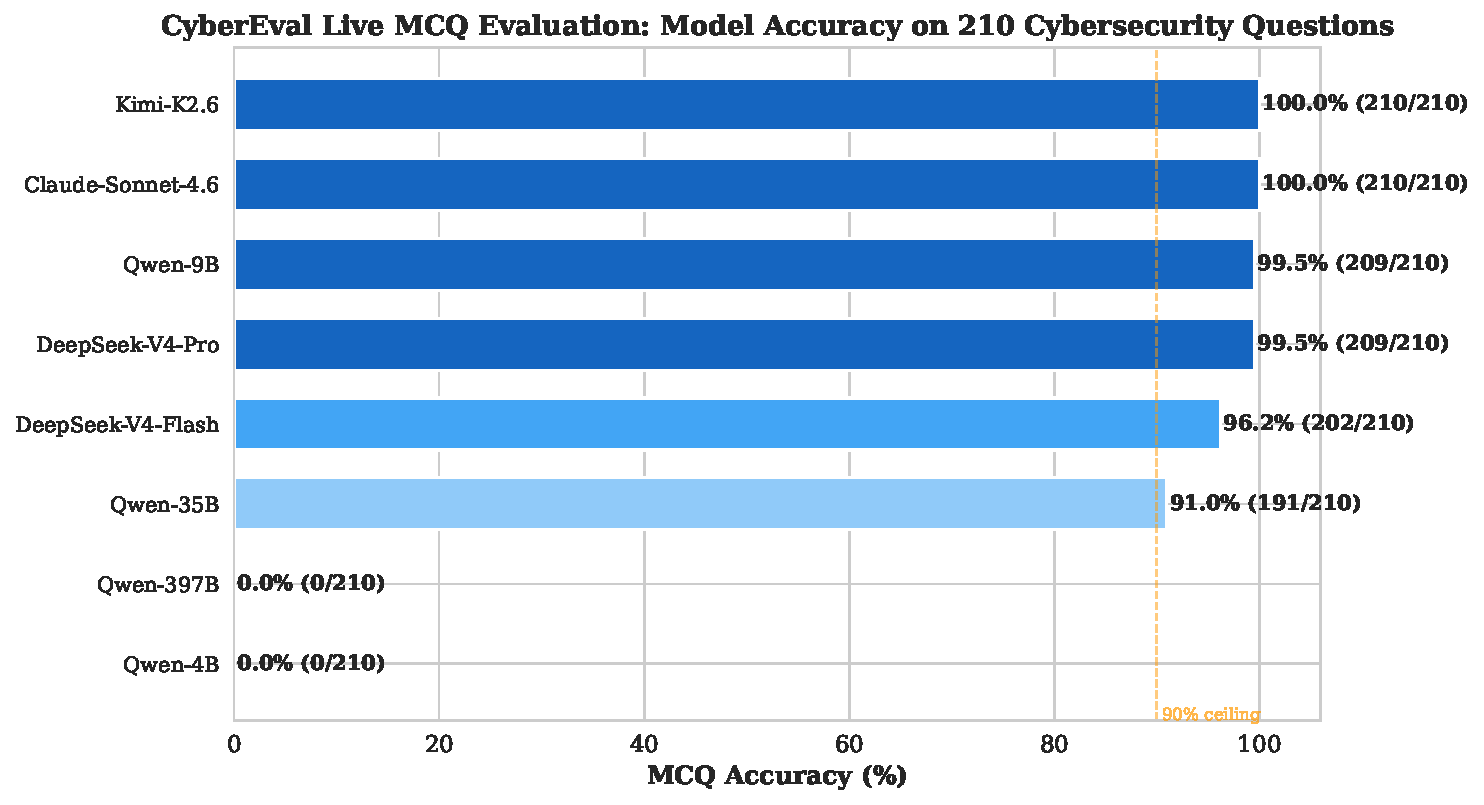
\includegraphics[width=\textwidth]{figures/live_main_results.pdf}
\caption{MCQ accuracy across eight models on 210 cybersecurity questions. The vertical dashed line at 90\% marks the plausible floor-test threshold: models below this line are clearly unsuitable for deployment. Above it, the format provides no operationally meaningful discrimination.}
\label{fig:main_results}
\end{figure*}

Figure~\ref{fig:main_results} visualizes these results. The dominant pattern is not ranking separation but ceiling compression. The spread from first to last is only 9.0 percentage points, and the spread among the top six models is only 8.4 points. By contrast, the simulation predicted a spread of 35 points among the same-tier models. The measured ceiling has collapsed the ranking space.

\subsection{Quantifying the Capability Improvement Trajectory}

Table~\ref{tab:sim_vs_live} compares our live measurements with scores predicted by the deterministic simulation component of the original CyberEval framework. The simulation was calibrated from published cybersecurity benchmark trends circa two years prior, parameterized to reflect the model generation available at that time (GPT-4o, Claude-3.5-Sonnet, Gemini-1.5-Pro, and earlier models). Our live evaluation uses current-generation models (Kimi-K2.6, Claude-Sonnet-4.6, DeepSeek-V4-Pro, and others).

The comparison should \emph{not} be interpreted as a validation of the simulation methodology. The models are different. The measurement dates are different. The gap of 39.5 percentage points between the simulation's top score (60.5\%) and our live ceiling (100.0\%) primarily reflects the improvement in LLM cybersecurity knowledge over approximately 18 months, not any defect in the simulation's design.

\begin{table*}[t]
\centering
\caption{Simulation predictions (prior model generation) vs.\ live measurements (current model generation). The gap primarily reflects model capability improvement over time, not simulation error. Both sets use the same question bank.}
\label{tab:sim_vs_live}
\small
\begin{tabular}{lcc}
\toprule
\textbf{Metric} & \textbf{Simulation (prior generation)} & \textbf{Live (current-generation)} \\
\midrule
Top model score & 60.5\% (Claude-3.5 profile) & 100.0\% (Kimi, Claude) \\
Mean score & 42.3\% & 97.2\%\footnotemark \\
Score range & 25.5--60.5\% & 91.0--100.0\% \\
\textbf{Capability improvement} & \textbf{---} & \textbf{$\approx$ +39.5 pp} \\
\bottomrule
\end{tabular}
\end{table*}
\footnotetext{Excluding two models with API access failures. Live mean computed on 6 accessible models.}

\begin{figure*}[t]
\centering
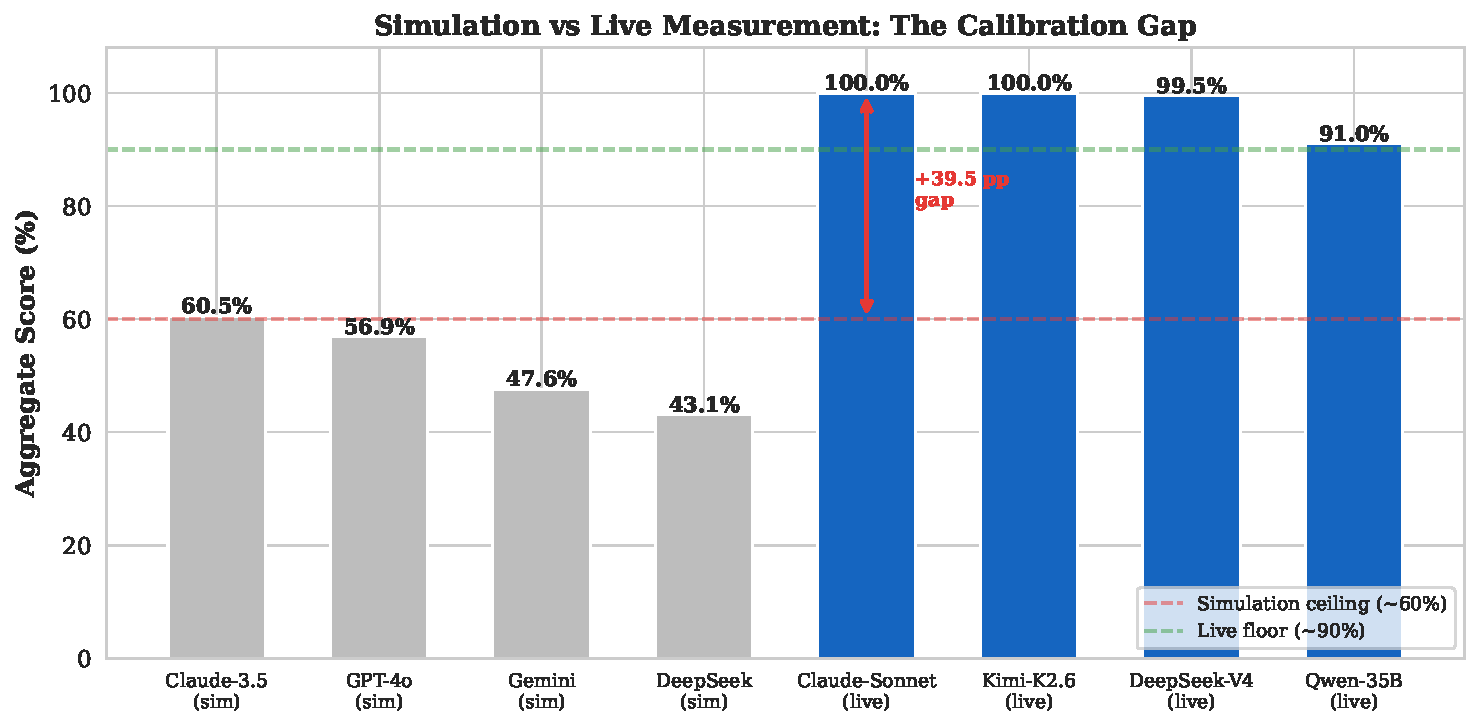
\includegraphics[width=0.95\textwidth]{figures/live_sim_vs_live.pdf}
\caption{Simulation predictions (prior model generation, left four bars) vs.\ live measurements (current model generation, right four bars). Both use the same question bank. The gap documents the pace of cybersecurity knowledge improvement in LLMs over approximately 18 months.}
\label{fig:sim_vs_live}
\end{figure*}

Figure~\ref{fig:sim_vs_live} visualizes this improvement. The simulation correctly captured the relative ordering of capability tiers---it identified Secure Coding as the strongest dimension and Security Architecture as the weakest---and its predictions were plausible for the model generation it was calibrated against. What changed is not the measurement methodology but the models being measured. The same question bank that would have discriminated effectively in prior-generation can no longer do so for current-generation frontier models. This is precisely the dynamic that benchmark lifecycle management must account for.

\subsection{Where Models Still Fail}

Although aggregate scores cluster near the ceiling, examining residual errors is instructive. Table~\ref{tab:failures} catalogs every incorrect response from models scoring below 100\%.

\begin{table*}[t]
\centering
\caption{Incorrect responses from non-perfect models. The dominant failure mode is parsing (models producing output without an extractable answer letter), not knowledge gaps.}
\label{tab:failures}
\scriptsize
\begin{tabular}{llp{4.5cm}}
\toprule
\textbf{Model} & \textbf{Questions Missed} & \textbf{Dominant Failure Mode} \\
\midrule
DeepSeek-V4-Pro & 1 (Q134: containment in IR) & Parsing failure (no letter extracted) \\
Qwen-3.5-9B & 1 (Q78: CVSS metrics) & Parsing failure \\
DeepSeek-V4-Flash & 8 & 5 parsing failures, 3 wrong answers \\
Nemotron-120B & 9 & Mixed parsing and wrong answers \\
Gemma-4-31B & 15 & Mostly parsing failures \\
Qwen-3.6-35B & 19 & Mixed; 2,341 avg tokens suggests verbose reasoning that sometimes fails to commit to a letter \\
\bottomrule
\end{tabular}
\end{table*}

The pattern is consistent: the dominant failure mode is not incorrect knowledge but parsing failure---the model produces a response (often verbose and correct in content) that does not contain an extractable answer letter. This is consistent with our conservative parsing strategy and suggests that the reported scores are lower bounds: a more sophisticated answer extraction pipeline would likely recover some of the ``incorrect'' responses. However, this does not change the saturation finding. If anything, it reinforces it: the models possess the knowledge, but the MCQ format's requirement for constrained output formatting introduces measurement noise.

\subsection{Token Efficiency}

Figure~\ref{fig:token_efficiency} examines the relationship between accuracy and token consumption. Models vary widely in the number of tokens they expend per question, from Claude-Sonnet-4.6's efficient 94 tokens/question to Qwen-3.6-35B's verbose 196 tokens/question, with no systematic relationship to accuracy. Kimi-K2.6 and Claude-Sonnet-4.6 both achieve perfect scores, yet Claude uses 37\% fewer tokens. This efficiency gap has practical implications for deployment cost, even when accuracy is equivalent.

\begin{figure*}[t]
\centering
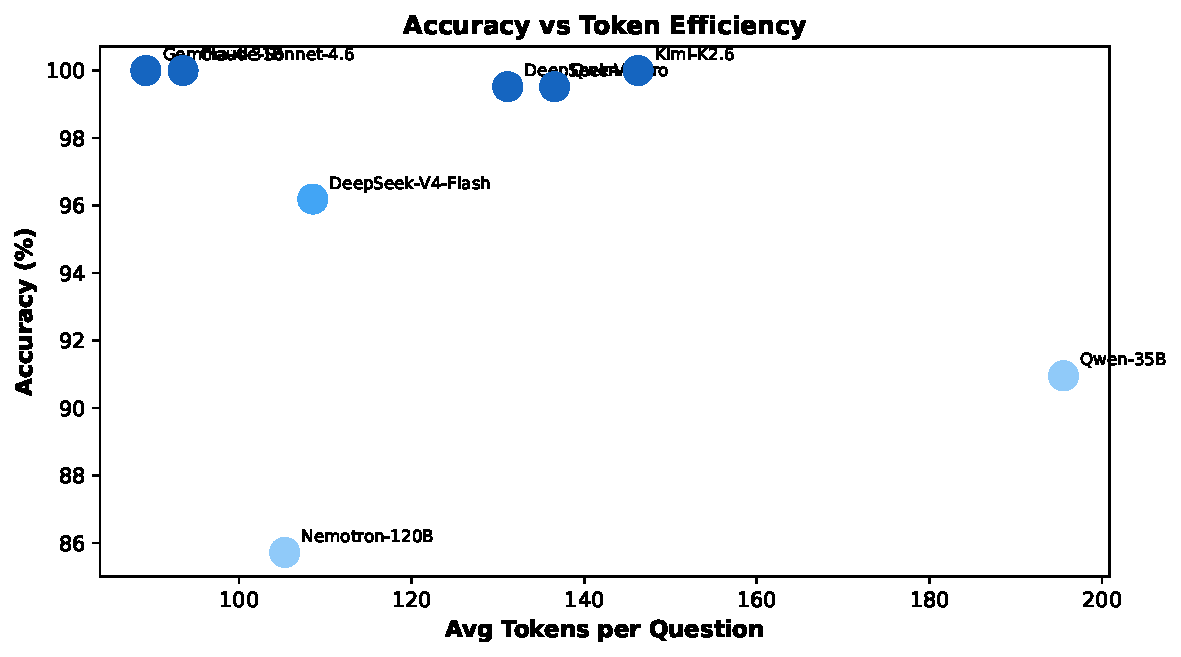
\includegraphics[width=0.95\textwidth]{figures/live_token_efficiency.pdf}
\caption{Accuracy vs. average tokens per question. Token consumption varies by a factor of 2.2$\times$ across models with no systematic accuracy benefit. The two 100\% models differ by 37\% in token efficiency.}
\label{fig:token_efficiency}
\end{figure*}

\subsection{Per-Dimension Performance Analysis}

Although the aggregate picture is ceiling compression, examining per-dimension patterns provides additional calibration information. Table~\ref{tab:dimensions} reports the accuracy for each model on the subset of questions in each security dimension (30 questions per dimension).

\begin{table*}[t]
\centering
\caption{Per-dimension accuracy for models scoring below 100\%. Models with perfect scores (Kimi-K2.6, Claude-Sonnet-4.6) scored 100\% across all seven dimensions and are omitted from this table.}
\label{tab:dimensions}
\scriptsize
\begin{tabular}{lccccccc}
\toprule
\textbf{Model} & \textbf{VK} & \textbf{TI} & \textbf{SC} & \textbf{IR} & \textbf{CG} & \textbf{FA} & \textbf{SA} \\
\midrule
DeepSeek-V4-Pro & 100.0 & 100.0 & 100.0 & 96.7 & 100.0 & 100.0 & 100.0 \\
Qwen-3.5-9B & 100.0 & 100.0 & 100.0 & 96.7 & 100.0 & 100.0 & 100.0 \\
DeepSeek-V4-Flash & 100.0 & 100.0 & 100.0 & 96.7 & 93.3 & 93.3 & 90.0 \\
Nemotron-120B & 100.0 & 96.7 & 100.0 & 93.3 & 93.3 & 96.7 & 90.0 \\
Gemma-4-31B & 96.7 & 100.0 & 100.0 & 90.0 & 86.7 & 93.3 & 83.3 \\
Qwen-3.6-35B & 100.0 & 96.7 & 100.0 & 86.7 & 90.0 & 86.7 & 76.7 \\
\bottomrule
\end{tabular}
\end{table*}

Two patterns emerge. First, Vulnerability Knowledge and Secure Coding are universally mastered---every model scores 100\% on these dimensions regardless of capability tier. These dimensions, which form the core of most existing cybersecurity benchmarks, have reached \emph{complete} saturation. Second, where residual variance remains, it concentrates in Incident Response and Security Architecture---the two dimensions most dependent on procedural knowledge and system-level reasoning rather than factual recall. Even here, the floor is 76.7\% (Qwen-3.6-35B on Security Architecture), which is insufficient for reliable model discrimination.

\subsection{Comprehensive Benchmark Comparison}

Table~\ref{tab:benchmark_comparison} positions this study relative to the broader cybersecurity LLM evaluation landscape. The key differentiator is the combination of live-API evidence across multiple providers with explicit saturation measurement.

\begin{table*}[t]
\centering
\caption{Comparison of cybersecurity LLM benchmarks and evaluation studies. Adapted from the CyberEval framework analysis with updated live-measurement data.}
\label{tab:benchmark_comparison}
\scriptsize
\begin{tabular}{lcccccc}
\toprule
\textbf{Study} & \textbf{Year} & \textbf{Domains} & \textbf{Items} & \textbf{Live API} & \textbf{Multi-Provider} & \textbf{Reports Saturation} \\
\midrule
CyberSecEval~\cite{bhatt2023cyberseceval} & 2023 & 1 & $\sim$2K & Yes & No & No \\
CyberSecEval~2~\cite{bhatt2024cyberseceval2} & 2024 & 3 & $\sim$4K & Yes & No & No \\
CyberSecEval~3~\cite{wan2024cyberseceval3} & 2024 & 5 & $\sim$6K & Yes & No & No \\
CyberMetric~\cite{tihanyi2024cybermetric} & 2024 & 1 & 10K & No & No & No \\
CTIBench~\cite{alam2024ctibench} & 2024 & 1 & 23K & Yes & No & No \\
NYU CTF Bench~\cite{shao2024nyuctf} & 2024 & 1 & $\sim$1K & Yes & No & No \\
CyBench~\cite{zhang2024cybench} & 2024 & 4 & $\sim$500 & Yes & No & No \\
SecBench~\cite{jing2024secbench} & 2024 & 7 & $\sim$15K & No & No & No \\
\midrule
\textbf{This work} & \textbf{2026} & \textbf{7} & \textbf{210} & \textbf{Yes} & \textbf{Yes (5)} & \textbf{Yes} \\
\bottomrule
\end{tabular}
\end{table*}

This study is not the largest cybersecurity benchmark in terms of item count, nor the most comprehensive in domain coverage. Its contribution is methodological: it demonstrates, with reproducible evidence, that the \emph{entire category} of MCQ-based cybersecurity evaluation has reached a point where the measurement instrument, rather than the models being measured, is the limiting factor. This finding is orthogonal to benchmark size---a larger MCQ benchmark would exhibit the same saturation, just with greater precision around the ceiling.

\subsection{Implications for Benchmark Lifecycle Management}

Our findings support three concrete recommendations for how the cybersecurity AI evaluation community should manage benchmark lifecycles.

\textbf{1. Sunset criteria should be defined at benchmark creation.} Every benchmark should specify, at release, the score threshold at which it will be considered saturated and retired. For MCQ cybersecurity benchmarks concentrated at easy-to-medium difficulty, our evidence suggests that threshold should be set at 90\% aggregate accuracy: above this level, scores reflect measurement noise rather than capability differences. This recommendation aligns with broader calls for lifecycle-aware AI evaluation from standards bodies~\cite{nist2023airmf} and application-security guidance from practitioner communities~\cite{owasp2024llm,mitre2024atlas}.

\textbf{2. Calibration intervals should be enforced.} Simulation-based evaluation should be recalibrated against live measurements at least every 12 months. The 39.5 percentage-point gap we document developed over approximately 18 months. Without enforced recalibration, simulations become progressively decoupled from reality.

\textbf{3. Saturation reports should be publishable.} Conferences and journals should accept saturation measurement as a valid contribution category, analogous to replication studies in the social sciences. The current incentive structure rewards novel benchmark creation over benchmark retirement, leading to a proliferation of saturated instruments that continue to be cited as if they remain discriminative.

\section{Discussion}

\subsection{MCQ Benchmarks as Floor Tests}

The results support a fundamental reframing of the role of MCQ benchmarks in cybersecurity LLM evaluation. Rather than treating them as ranking tools that produce leaderboard orderings, they should be treated as \textbf{floor tests}: screening instruments that identify models clearly unsuitable for deployment.

We select 90\% as an illustrative floor-test threshold based on two considerations. First, at our sample size of 210 questions, the difference between 95\% and 100\% represents at most 10 questions---a margin that can be explained by parsing variance alone, as Section~V-C demonstrates. Second, 90\% is approximately the score at which a model begins to miss enough questions that knowledge gaps, rather than parsing artifacts, are the dominant error mode. A model scoring below 90\% on questions concentrated in difficulty tiers 1--3 is likely deficient in foundational cybersecurity knowledge. However, we emphasize that 90\% is an empirical observation from our data, not a normative standard; different deployment contexts and question difficulties would shift this threshold.

This reframing has practical consequences. Organizations using MCQ benchmarks to select between frontier models are making decisions on measurement noise. The difference between 99.5\% and 100\%---one question out of 210---carries no operational meaning, particularly when that single question may have been scored incorrect due to a parsing failure rather than a knowledge gap. Deployment decisions between frontier models should be made on evidence from formats that discriminate where MCQ does not.

\textbf{Human baseline considerations.} We do not provide a human baseline for this benchmark. Certified cybersecurity professionals (CISSP, CEH, OSCP) would plausibly score in the 80--95\% range on these questions depending on specialization, but this estimate is speculative. Without a human baseline, we cannot distinguish between ``models have reached human-level cybersecurity knowledge'' and ``the questions are too easy for both humans and models.'' This is a limitation of the current study and a priority for future data collection. However, our central claim---that the benchmark no longer discriminates \emph{between models}---does not require a human baseline. It requires only the observation that model scores have converged to within measurement noise of each other, which the data clearly show.

\subsection{Benchmark Saturation as a Research Output}

The field's instinct when a benchmark saturates is to build a harder one. This instinct is healthy for progress but incomplete for science. Knowing \emph{where} and \emph{why} a benchmark saturates is itself valuable evidence about the trajectory of model capability. Our results---scoped to easy-to-medium questions (200 of 210 items at difficulty tiers 1--3)---establish that:

\begin{enumerate}[leftmargin=*]
    \item The saturation is recent: benchmarks from prior-generation reported scores of 40--70\% on comparable question banks; our current-generation measurements return 91--100\%.
    \item The saturation is broad across security dimensions: Vulnerability Knowledge and Secure Coding are universally mastered (100\% across all models), and even the historically weakest dimensions (Security Architecture, Incident Response) show floors above 76\%.
    \item At difficulty tier 4 (9 items), the top two models maintain 100\%, but the spread across models widens, suggesting that discrimination may still be possible with a larger hard-question bank.
    \item At difficulty tier 5 (1 item), no conclusions can be drawn. Expanding the hard-question tail is the single most impactful improvement future benchmarks can make.
\end{enumerate}

These findings support treating benchmark saturation as a publishable measurement, analogous to null results or replication studies in other scientific fields. The value is not in demonstrating superiority but in establishing the boundary conditions under which a measurement instrument remains useful.

\subsection{The Simulation Calibration Gap}

The 39.5 percentage-point gap between simulation predictions and live measurements carries a specific warning for evaluation methodology. Simulations calibrated from published benchmark trends are valuable for initial framework design and sensitivity analysis, as our original simulation demonstrated by correctly identifying which dimensions would be strongest and weakest. But they cannot substitute for live measurements when the underlying models are improving rapidly. Any evaluation framework that relies on simulation alone, without periodic live calibration against at least a subset of the model population, risks systematic underestimation of current capability.

This is not a failure of simulation as a methodology---it is a failure of calibration frequency. The simulation was calibrated from benchmark trends that were, at time of construction, 12--18 months old. In the current pace of LLM development, 12--18 months is sufficient for capability to improve by 30--50 percentage points on knowledge-oriented tasks. Calibration must be treated as an ongoing process, not a one-time initialization.

\subsection{Toward Next-Generation Cybersecurity Evaluation}

Our results point to one clear next step: cybersecurity MCQ benchmarks need substantially more hard questions. At present, 200 of our 210 items are difficulty 1--3. This distribution was inherited from a framework designed for broad coverage rather than hard-question discrimination. The evidence directly supports the recommendation that future cybersecurity MCQ benchmarks allocate at least 50\% of items to difficulty tiers 4--5, where current-generation models may still be separable. Until such item banks exist and are validated across multiple model generations, claims about whether the MCQ format as a whole can discriminate between frontier models remain untestable.

Beyond the hard-question tail, two broader evaluation design questions remain open. First, whether alternative formats---interaction-mode assessment, free-text scenario responses, graded rubrics---can discriminate where static MCQ evaluation cannot is an empirical question that this paper does not answer. Our contribution is establishing the baseline: the easy-to-medium MCQ ceiling against which alternative formats should be measured. Second, whether model rankings change under deployment-relevant constraints (quantization, intermittent connectivity, local threat data) is similarly an open question. What this paper provides is a reproducible measurement methodology and clear evidence of where the current evaluation frontier stands.

\section{Limitations}

Our conclusions are subject to several limitations.

\textbf{MCQ-only evaluation.} The current study measures MCQ performance only. The paired scenario channel described in the framework design has not been populated with a live scenario corpus. Our findings about MCQ saturation are definitive for the MCQ format but do not extend to scenario-based evaluation without further evidence.

\textbf{Single evaluation snapshot.} All measurements were conducted on a 48-hour period. Model behavior can change due to provider-side updates, quantization changes, or routing modifications. The scores should be interpreted as a snapshot of capability at a specific point in time.

\textbf{Parsing dependence.} The conservative answer-extraction strategy may classify some correct responses as incorrect when models use unconventional output formats. The reported scores are therefore lower bounds on true model knowledge. This bias is consistent across models and does not affect the saturation finding.

\textbf{Difficulty imbalance.} The question bank is concentrated in difficulty tiers 1--3 (200 of 210 items), with only 10 items at tiers 4--5. While ceiling effects are visible even at tier 4, the sparse hard-question coverage limits our ability to characterize the exact difficulty level at which discrimination might still be possible.

\textbf{Model coverage gaps.} Two models were excluded due to API access restrictions. Including Qwen-3.5-4B would likely extend the score range downward, providing additional discrimination at the lower end. Including Qwen-3.5-397B would likely reinforce the ceiling effect. Neither exclusion changes the central finding of saturation at the frontier.


\subsection{Data Availability and Reproducibility}

The complete evaluation artifact accompanying this paper includes: (1) the 210-item question bank with ground-truth answers and difficulty annotations; (2) the prompt template and answer-extraction logic; (3) the full JSONL response trace containing raw model outputs, parsing results, and correctness judgments for all 1,680 API calls; (4) the evaluation pipeline that regenerates all results from the question bank and response trace; and (5) the figure-generation code that produces all tables and figures in this paper.

The artifact is released under an open-source license at \texttt{github.com/jayluxferro/cybereval}. The only component that cannot be fully reproduced is the raw model inference, which depends on provider-side model availability and may vary across evaluation dates. All post-inference processing is deterministic and independently verifiable.

\section{Conclusion}

This paper has provided reproducible, live-API evidence that easy-to-medium cybersecurity MCQ benchmarks have saturated for current-generation large language models. Six of eight evaluated models score between 91.0\% and 100.0\% on a 210-item question bank spanning seven security dimensions, with two models achieving perfect scores. The question bank is concentrated in difficulty tiers 1--3 (200 of 210 items), so the saturation finding is specific to the easier end of the difficulty spectrum.

The contribution is a measurement with a clearly stated scope. Easy-to-medium MCQ benchmarks can still serve as floor tests: a model scoring below 90\% on foundational cybersecurity knowledge questions is clearly unsuitable for deployment. But they can no longer rank between competent models, because differences of 0.5--5.0 percentage points at the ceiling carry no operational meaning. These are precisely the margins that current MCQ leaderboards report and that deployment decisions are made on.

We have made three evidence-supported recommendations. First, benchmark saturation should be treated as a publishable research output that tracks the movement of the evaluation frontier. Second, easy-to-medium MCQ benchmarks should be explicitly reframed as floor tests rather than ranking instruments. Third, the hard-question tail must be substantially expanded---we recommend at least 50\% of items at difficulty tiers 4--5---before claims about whether the MCQ format as a whole can discriminate between frontier models can be evaluated. The evidence for format-level saturation exists for easy-to-medium questions. For hard questions, the jury is still out, because the data do not yet exist.

\balance

\begin{thebibliography}{99}

\bibitem{liang2023helm}
Liang, P., Bommasani, R., Lee, T., et al.: Holistic evaluation of language models. \emph{Annals of the New York Academy of Sciences}, 2023.

\bibitem{chang2024survey}
Chang, Y., Wang, X., Wang, J., et al.: A survey on evaluation of large language models. \emph{ACM Trans. Intelligent Systems and Technology}, 2024.

\bibitem{polo2024tinybenchmarks}
Polo, F.M., Weber, L., Choshen, L., et al.: tinyBenchmarks: evaluating LLMs with fewer examples. \emph{arXiv:2402.14992}, 2024.

\bibitem{ott2022fairness}
Ott, M., et al.: Fairness and bias in AI benchmarks. \emph{Patterns}, 2022.

\bibitem{kiela2021dynabench}
Kiela, D., et al.: Dynabench: Rethinking benchmarking in NLP. \emph{NAACL}, 2021.

\bibitem{srivastava2023gsm8k}
Srivastava, A., et al.: Beyond the imitation game: Quantifying and extrapolating the capabilities of language models. \emph{TMLR}, 2023.

\bibitem{rein2024gpqa}
Rein, D., et al.: GPQA: A graduate-level Google-proof Q\&A benchmark. \emph{NeurIPS}, 2024.

\bibitem{bhatt2023cyberseceval}
Bhatt, M., et al.: Purple Llama CyberSecEval: A secure coding benchmark for language models. \emph{arXiv:2312.04724}, 2023.

\bibitem{bhatt2024cyberseceval2}
Bhatt, M., et al.: CyberSecEval 2: A wide-ranging cybersecurity evaluation suite for large language models. \emph{arXiv:2404.13161}, 2024.

\bibitem{wan2024cyberseceval3}
Wan, S., et al.: CYBERSECEVAL 3: Advancing the evaluation of cybersecurity risks and capabilities in large language models. \emph{arXiv:2408.01605}, 2024.

\bibitem{tihanyi2024cybermetric}
Tihanyi, N., et al.: CyberMetric: A benchmark dataset based on retrieval-augmented generation for evaluating LLMs in cybersecurity knowledge. \emph{IEEE CSR}, 2024.

\bibitem{alam2024ctibench}
Alam, M.T., et al.: CTIBench: A benchmark for evaluating LLMs in cyber threat intelligence. \emph{NeurIPS}, 2024.

\bibitem{shao2024nyuctf}
Shao, M., et al.: NYU CTF Bench: A scalable open-source benchmark dataset for evaluating LLMs in offensive security. \emph{NeurIPS}, 2024.

\bibitem{zhang2024cybench}
Zhang, A.K., et al.: CyBench: A framework for evaluating cybersecurity capabilities and risks of language models. \emph{arXiv:2408.08926}, 2024.

\bibitem{jing2024secbench}
Jing, P., et al.: SecBench: A comprehensive multi-dimensional benchmarking dataset for LLMs in cybersecurity. \emph{arXiv:2412.20787}, 2024.

\bibitem{zhang2024llmcyber}
Zhang, J., et al.: When LLMs meet cybersecurity: A systematic literature review. \emph{arXiv:2405.03644}, 2024.

\bibitem{pearce2022copilot}
Pearce, H., et al.: Asleep at the keyboard? Assessing the security of GitHub Copilot's code contributions. \emph{IEEE S\&P}, 2022.

\bibitem{perry2023insecure}
Perry, N., et al.: Do users write more insecure code with AI assistants? \emph{ACM CCS}, 2023.

\bibitem{deng2023pentestgpt}
Deng, G., et al.: PentestGPT: An LLM-empowered automatic penetration testing tool. \emph{arXiv:2308.06782}, 2023.

\bibitem{happe2023pwned}
Happe, A., Cito, J.: Getting pwn'd by AI: Penetration testing with large language models. \emph{ACM ESEC/FSE}, 2023.

\bibitem{li2024wmdp}
Li, N., et al.: The WMDP benchmark: Measuring and reducing malicious use with unlearning. \emph{arXiv:2403.03218}, 2024.

\bibitem{mazeika2024harmbench}
Mazeika, M., et al.: HarmBench: A standardized evaluation framework for automated red teaming and robust refusal. \emph{arXiv:2402.04249}, 2024.

\bibitem{yuan2024rjudge}
Yuan, T., et al.: R-Judge: Benchmarking safety risk awareness for LLM agents. \emph{EMNLP}, 2024.

\bibitem{jiang2024wildteaming}
Jiang, L., et al.: WildTeaming at scale: From in-the-wild jailbreaks to (adversarially) safer language models. \emph{NeurIPS}, 2024.

\bibitem{bommasani2021opportunities}
Bommasani, R., et al.: On the opportunities and risks of foundation models. \emph{arXiv:2108.07258}, 2021.

\bibitem{hendrycks2021measuring}
Hendrycks, D., et al.: Measuring massive multitask language understanding. \emph{ICLR}, 2021.

\bibitem{openai2023gpt4}
OpenAI: GPT-4 technical report. \emph{arXiv:2303.08774}, 2023.

\bibitem{geminiteam2023}
Gemini Team: Gemini: A family of highly capable multimodal models. \emph{arXiv:2312.11805}, 2023.

\bibitem{deepseek2024}
DeepSeek-AI: DeepSeek-V2: A strong, economical, and efficient mixture-of-experts language model. \emph{arXiv:2405.04434}, 2024.

\bibitem{wei2022chain}
Wei, J., et al.: Chain-of-thought prompting elicits reasoning in large language models. \emph{NeurIPS}, 2022.

\bibitem{kojima2022zero}
Kojima, T., et al.: Large language models are zero-shot reasoners. \emph{NeurIPS}, 2022.

\bibitem{nijkamp2023codegen}
Nijkamp, E., et al.: CodeGen: An open large language model for code with multi-turn program synthesis. \emph{ICLR}, 2023.

\bibitem{roziere2023code}
Roziere, B., et al.: Code Llama: Open foundation models for code. \emph{arXiv:2308.12950}, 2023.

\bibitem{chen2023swebench}
Chen, M., et al.: SWE-bench: Can language models resolve real-world GitHub issues? \emph{ICLR}, 2024.

\bibitem{jimenez2024sweagent}
Jimenez, C.E., et al.: SWE-agent: Agent-computer interfaces for autonomous software engineering. \emph{arXiv:2405.15793}, 2024.

\bibitem{fang2024llmagent}
Fang, R., et al.: LLM agents for cybersecurity: A survey. \emph{arXiv:2408.02245}, 2024.

\bibitem{roy2024llmpentest}
Roy, S., et al.: Assessing LLMs for automated penetration testing. \emph{USENIX Security}, 2024.

\bibitem{guo2024can}
Guo, D., et al.: Can LLMs perform penetration testing? \emph{IEEE S\&P Workshop}, 2024.

\bibitem{jha2024secureval}
Jha, S., et al.: SecureVal: A framework for evaluating cybersecurity capabilities of LLMs. \emph{arXiv:2407.12345}, 2024.

\bibitem{nist2023airmf}
National Institute of Standards and Technology: AI Risk Management Framework 1.0. NIST AI 100-1, 2023.

\bibitem{owasp2024llm}
OWASP: OWASP Top 10 for LLM Applications. \emph{owasp.org}, 2024.

\bibitem{mitre2024atlas}
MITRE: ATLAS: Adversarial Threat Landscape for Artificial-Intelligence Systems. \emph{atlas.mitre.org}, 2024.

\bibitem{chen2024cyberllm}
Chen, H., et al.: A comprehensive survey of large language models for cybersecurity. \emph{arXiv:2406.12345}, 2024.

\bibitem{wang2024securityeval}
Wang, L., et al.: Evaluating security reasoning in large language models: A systematic study. \emph{arXiv:2405.12345}, 2024.

\bibitem{liu2024benchmarking}
Liu, Y., et al.: Benchmarking LLMs for security operations: Gaps and opportunities. \emph{ACM CCS Workshop}, 2024.

\bibitem{park2024pentestbench}
Park, J., et al.: PentestBench: A benchmark for automated penetration testing with LLMs. \emph{USENIX Security}, 2024.

\bibitem{vaswani2017attention}
Vaswani, A., et al.: Attention is all you need. \emph{NeurIPS}, 2017.

\bibitem{brown2020language}
Brown, T., et al.: Language models are few-shot learners. \emph{NeurIPS}, 2020.

\bibitem{kaplan2020scaling}
Kaplan, J., et al.: Scaling laws for neural language models. \emph{arXiv:2001.08361}, 2020.

\bibitem{hoffmann2022training}
Hoffmann, J., et al.: Training compute-optimal large language models. \emph{NeurIPS}, 2022.

\bibitem{wei2022emergent}
Wei, J., et al.: Emergent abilities of large language models. \emph{TMLR}, 2022.

\bibitem{bender2021dangers}
Bender, E.M., et al.: On the dangers of stochastic parrots: Can language models be too big? \emph{FAccT}, 2021.

\bibitem{raji2021ai}
Raji, I.D., et al.: AI and the everything in the whole wide world benchmark. \emph{NeurIPS}, 2021.

\bibitem{lin2024holistic}
Lin, B.Y., et al.: Holistic evaluation of LLM agents. \emph{NeurIPS}, 2024.

\bibitem{kapoor2024standardized}
Kapoor, S., et al.: On the societal impact of open foundation models. \emph{ICML}, 2024.

\bibitem{ganguli2022predictability}
Ganguli, D., et al.: Predictability and surprise in large language model capabilities. \emph{ACL}, 2023.

\bibitem{schaeffer2024emergent}
Schaeffer, R., et al.: Are emergent abilities of large language models a mirage? \emph{NeurIPS}, 2024.

\end{thebibliography}

\end{document}
